\subsection{Analyisis}


\begin{figure}[ht]
	\centering
	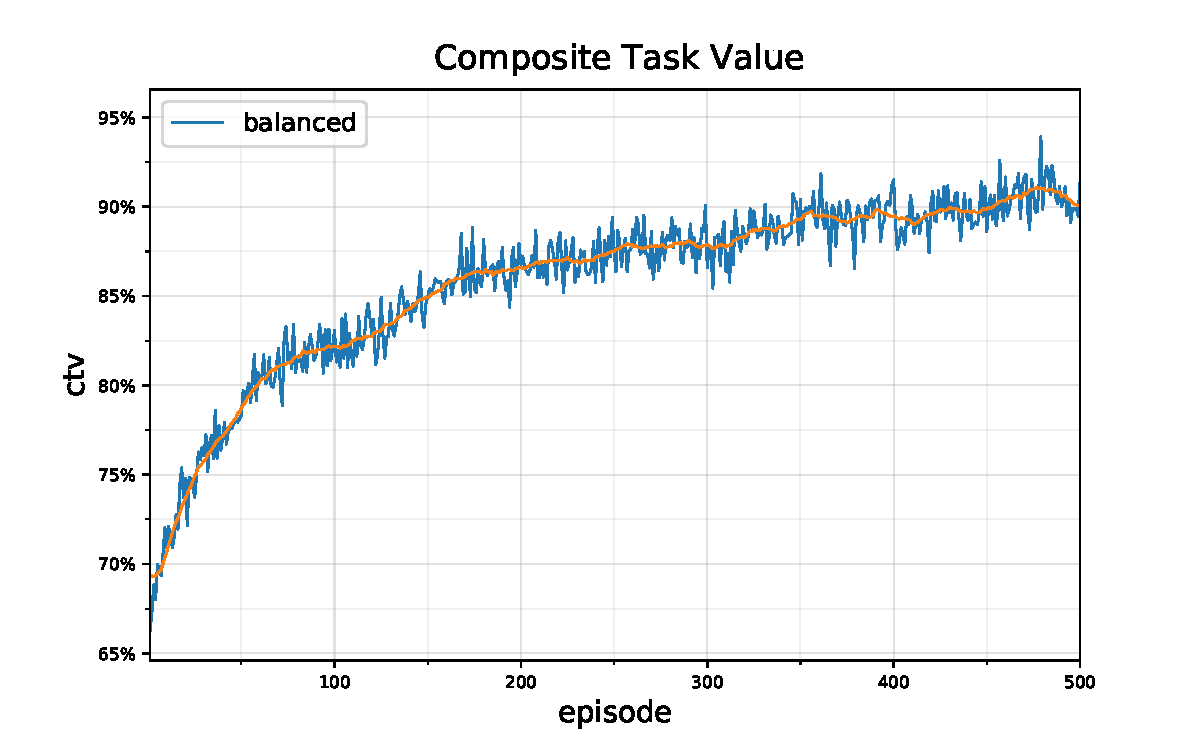
\includegraphics[width=0.7\linewidth]{5_ctv-optimal-ctv}
	\captionsetup{labelfont=bf,singlelinecheck=on}
	\caption{System utility compared to the theoretical maximum for the \simulationSimple{}{} system. The algorithms work to increase this value, which impacts the task values, energy consumption, and distribution depending on the weighting given to those various components}
	\label{fig:5_ctv-optimal-ctv}
\end{figure}
\begin{figure}[ht]
	\centering
	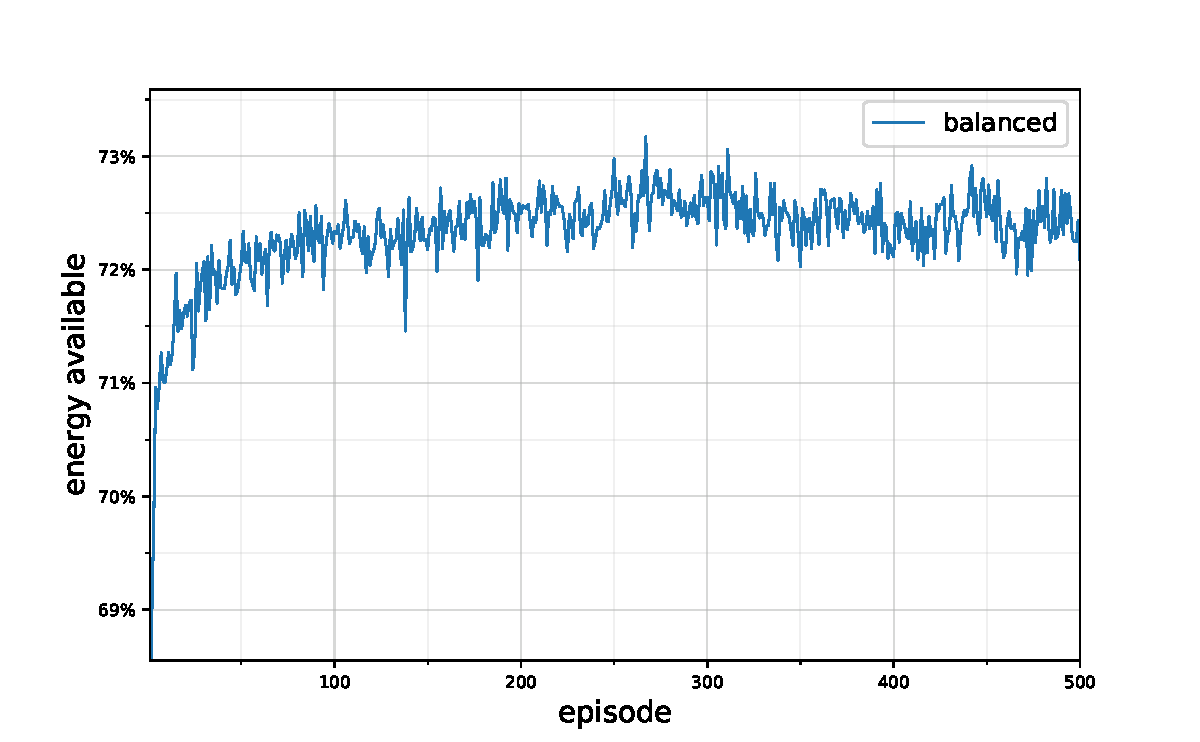
\includegraphics[width=0.7\linewidth]{5_ctv-statistics-energy-available}
	\captionsetup{labelfont=bf,singlelinecheck=on}
	\caption{Energy available in the \simulationSimple{}{} system as percentage of the maximum possible. Higher values show a more efficient use of agents to complete tasks, but may not give the best task values overall}
	\label{fig:5_ctv-statistics-energy-available}
\end{figure}
\begin{figure}[ht]
	\centering
	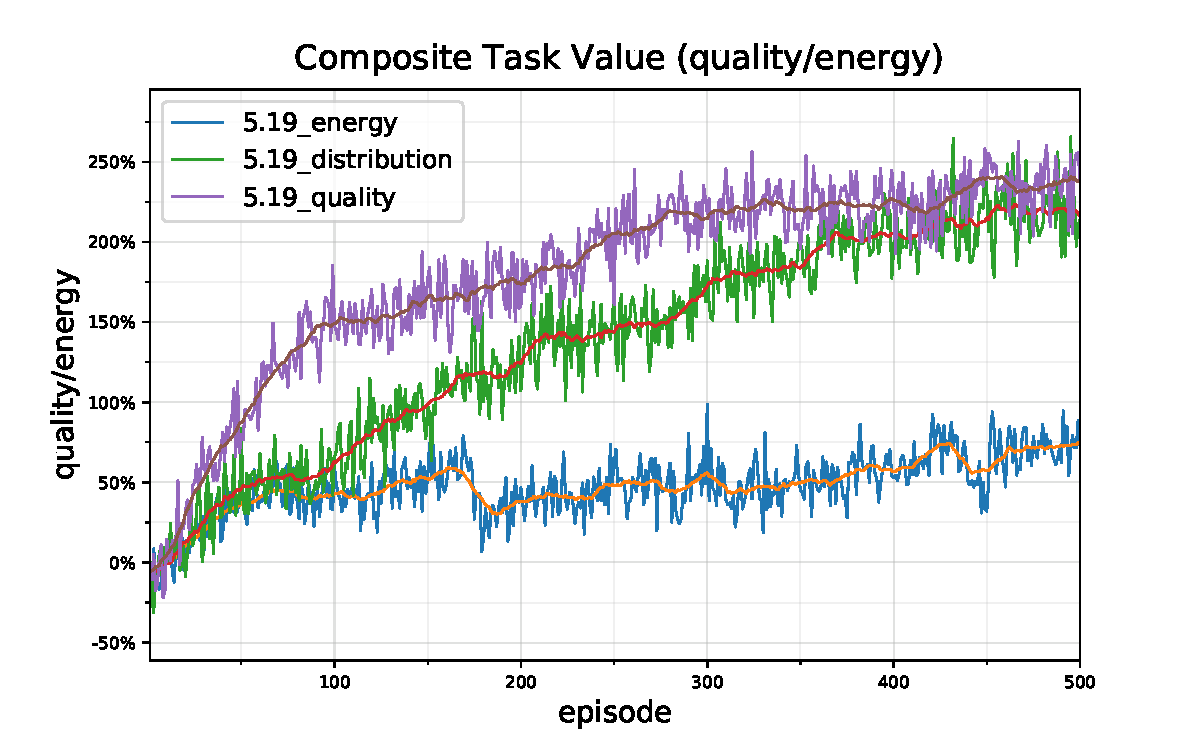
\includegraphics[width=0.8\linewidth]{5.19_ctv-quality-energy}
	\captionsetup{labelfont=bf,singlelinecheck=on}
	\caption{Quality/Energy available fraction for the \simulationExtended{}{} system. Higher values show dominance of task value in the CTV, lower values better energy consumption optimisation}
	\label{fig:5.19_ctv-quality-energy}
\end{figure}

\begin{figure}[ht]
	\centering
	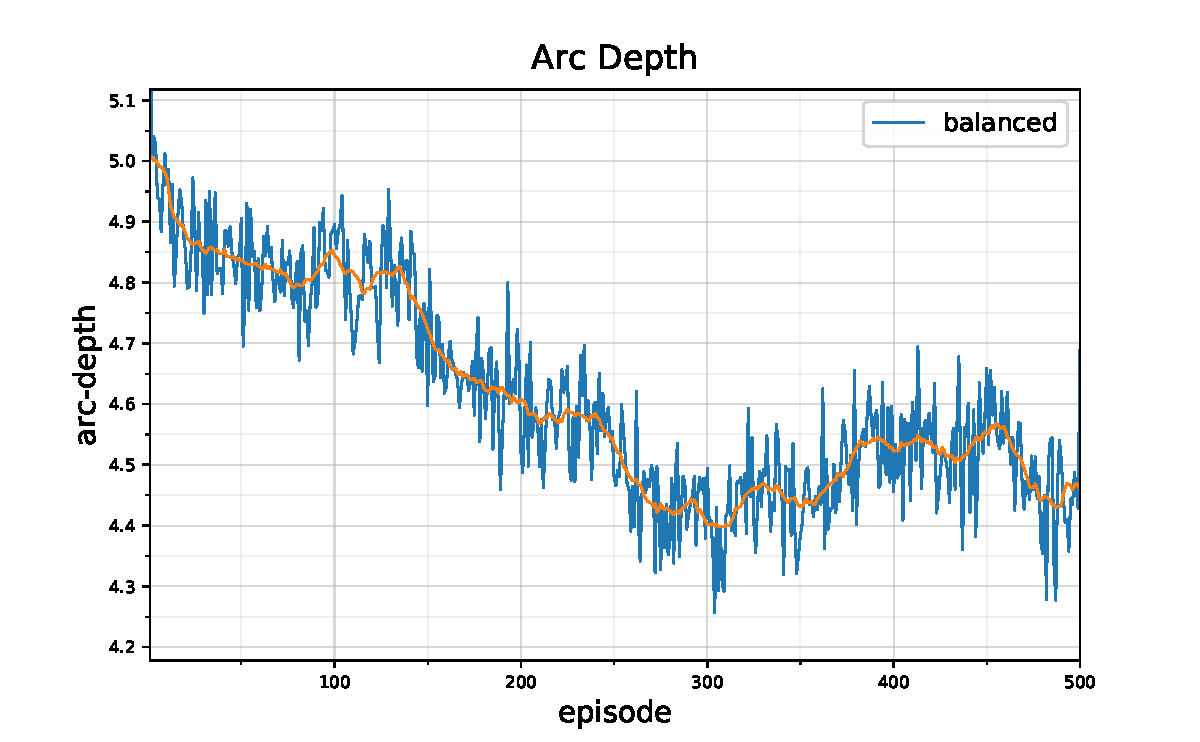
\includegraphics[width=0.7\linewidth]{5_ctv-arc-depth}
	\captionsetup{labelfont=bf,singlelinecheck=on}
	\caption{The average depth of arcs in the \simulationSimple{}{} system. Longer arcs allow sink agents to reach sensing agents that are closer to the task demand point, at the cost of greater energy usage}
	\label{fig:5_ctv-arc-depth}
\end{figure}
\begin{figure}[ht]
	\centering
	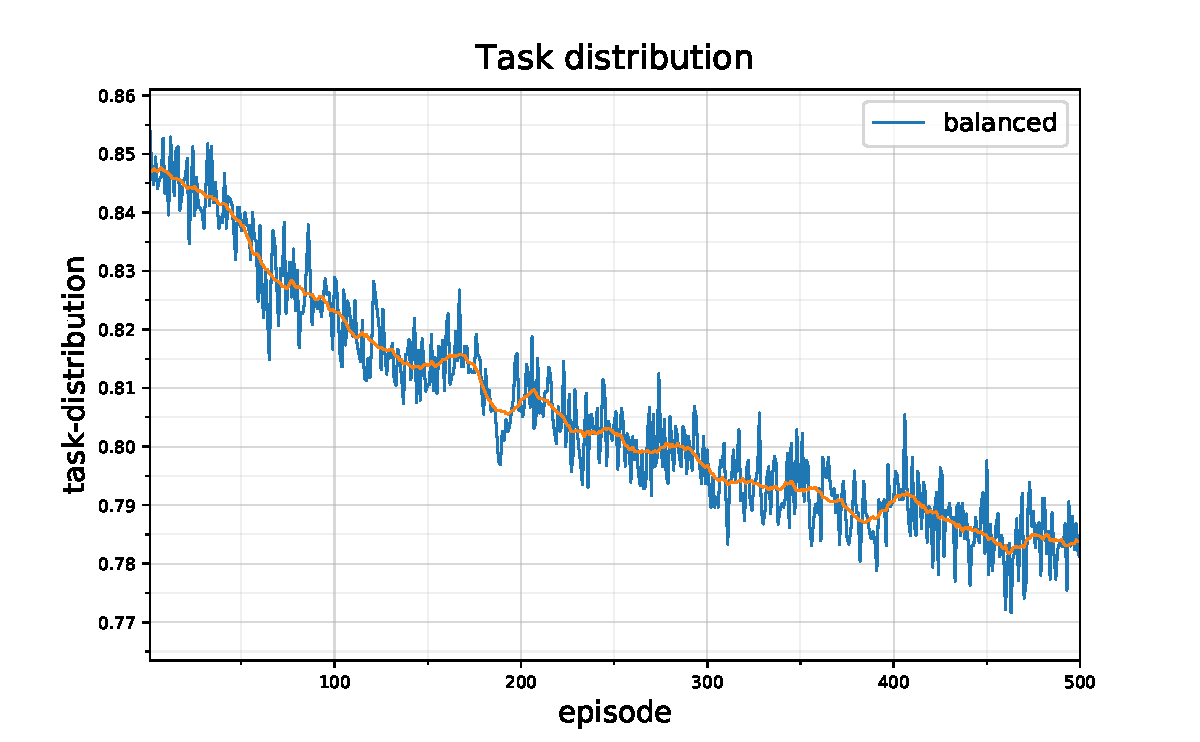
\includegraphics[width=0.7\linewidth]{5_ctv-task-distribution}
	\captionsetup{labelfont=bf,singlelinecheck=on}
	\caption{The task distribution in the system. Higher values spread energy usage across the system better, increasing the systems' lifetime}
	\label{fig:5_ctv-task-distribution}
\end{figure}
